% Drawing 154/01-7 -- folder 154, batch 01, archive page 13 (PDF page 14).
% Transcription: figure : l'arrangement standard de quatre pseudo-droites (orange) avec la droite jaune $D$ ; quatre régions portent le chiffre $4$ (quadrilatères). $\mathrm{St}_4$ est lu d'après la page ; il désigne vraisemblablement le système standard de $4$ pseudo-droites
% Kind: standard arrangement of four pseudolines with a line D. Method 2 (schematic redraw from the facsimile). Status: ok.
% Notes: Four orange pseudolines (the standard system St_4: they cross pairwise, two crossings above, one on, and three below the yellow line) and the yellow line D through the middle crossing, marked by a point; four regions carry the figure 4. Faint pencil doublings of two strands are drawn grey. The pairwise crossings are drawn as on the page; the arrangement is not encoded because two of the crossings near the bottom are hidden by the overlap of strokes.
% Coordinates: 1 unit = 1 mm = 1/100 of the crop width (bbox in page fractions: [0.121, 0.368, 0.284, 0.531]).
% Redrawn by Claude (claude-opus-5-5), issue #73, 2026-11-07; not checked by a human; not compiled (no TeX in the session).
% Rights: reproduces part of the work -- behind RENDER_TRANSCRIPTS, never published by itself.
\documentclass[tikz,border=3pt]{standalone}
\usepackage{amsmath,amssymb}
\usetikzlibrary{patterns,arrows.meta}
\tikzset{Or/.style={orange!90!black}, Ye/.style={yellow!80!orange}, Lg/.style={green!60!black!70}, Dg/.style={green!45!black}, Br/.style={brown!80!black}, Rd/.style={red!85!black}, Bl/.style={blue!70!black}, Gy/.style={black!40}, pencil/.style={black!45}, struck/.style={black!35}, mark/.style={circle,draw,inner sep=1.3pt}, pt/.style={circle,fill,inner sep=0.9pt}, opt/.style={circle,draw,fill=white,inner sep=1.1pt}}
\begin{document}
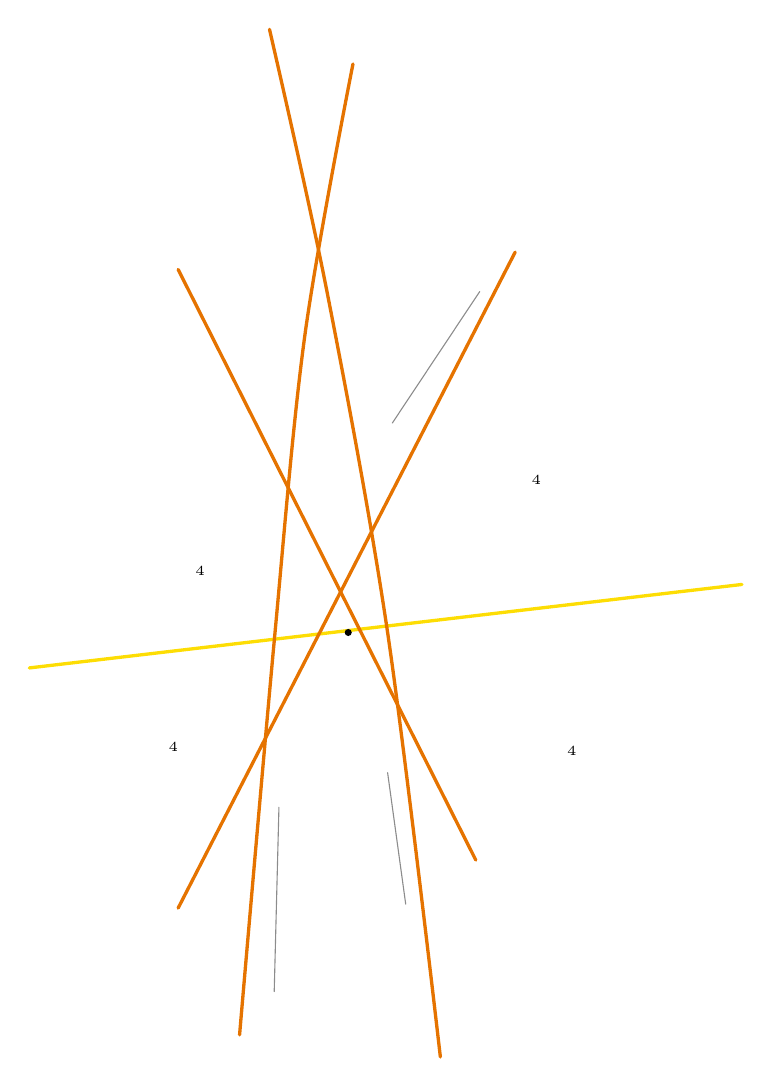
\begin{tikzpicture}[x=1mm,y=1mm,line cap=round,line join=round,font=\scriptsize]
\draw[Ye,very thick] (3.9,-86.7) -- (94.4,-76.1);
\node[pt] at (44.4,-82.2) {};
\draw[Or,very thick] plot[smooth, tension=0.55] coordinates {(34.4,-5.6) (41.7,-38.9) (49.4,-82.2) (56.1,-136.1)};
\draw[Or,very thick] plot[smooth, tension=0.55] coordinates {(45,-10) (38.9,-44.4) (35,-83.3) (30.6,-133.3)};
\draw[Or,very thick] (22.8,-36.1) -- (60.6,-111.1);
\draw[Or,very thick] (65.6,-33.9) -- (22.8,-117.2);
\draw[pencil] (35.6,-104.4) -- (35,-127.8);
\draw[pencil] (49.4,-100) -- (51.7,-116.7);
\draw[pencil] (61.1,-38.9) -- (50,-55.6);
\node[inner sep=1pt] at (25.6,-74.4) {\tiny $4$};
\node[inner sep=1pt] at (68.3,-62.8) {\tiny $4$};
\node[inner sep=1pt] at (22.2,-96.7) {\tiny $4$};
\node[inner sep=1pt] at (72.8,-97.2) {\tiny $4$};
\end{tikzpicture}
\end{document}
